\section{Evaluation}
\label{sec:evaluation}

\subsection{Experiments}

For tests was used a desktop Intel i5 4-Core @ 3.2GHz, while reading from a TTree with 100 million float values. We test three different use cases: GetBulkEntries, TTreeReaderFast and RDataSource.

\subsection{Results}

Figure \ref{fig:tbranch} shows the time spent on iterating all events in the \textit{TTree} with \textit{GetEntry} and \textit{GetBulkEntries}. Figure \ref{fig:ttreereader} shows the read time between \textit{TTreeReader} and \textit{TTreeReaderFast}. As shown in the figures, Bulk IO spends 10+ times less than \textit{GetEntry} and \textit{TTreeReader}. Bulk IO in both use cases spends similar time on reading events. \textit{TTreeReader} interface spends more than 3 times reading events than \textit{GetEntry} due to the overheads of TTreeReader itself (TTreeReader internally calls \textit{GetEntry}). 

\begin{figure}[!ht]
\centering
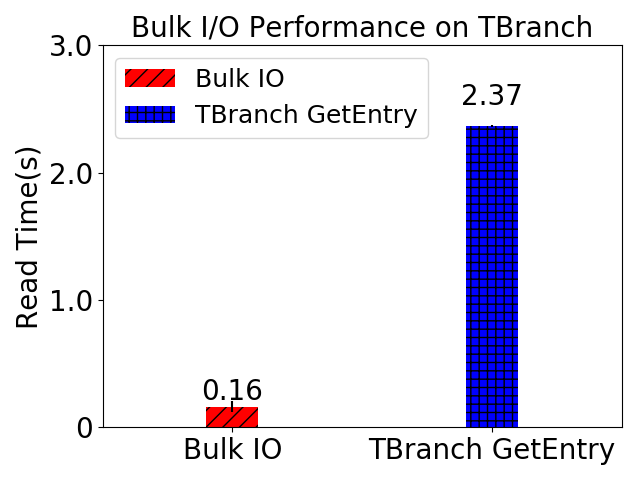
\includegraphics[height=4in, width=5in]{getbulkentries.png}
\vspace*{-2mm}
\caption{Performance between \textit{GetEntry} and \textit{GetBulkEntries}.}
\label{fig:tbranch}
\end{figure}

\begin{figure}[!ht]
\centering
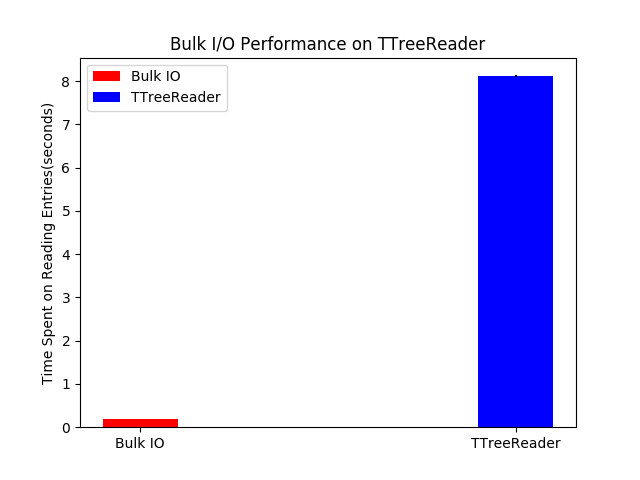
\includegraphics[height=4in, width=5in]{ttreereader.png}
\vspace*{-2mm}
\caption{Performance comparison between \textit{TTreeReader} and \textit{TTreeReaderFast}.}
\label{fig:ttreereader}
\end{figure}

\begin{figure}[!ht]
\centering
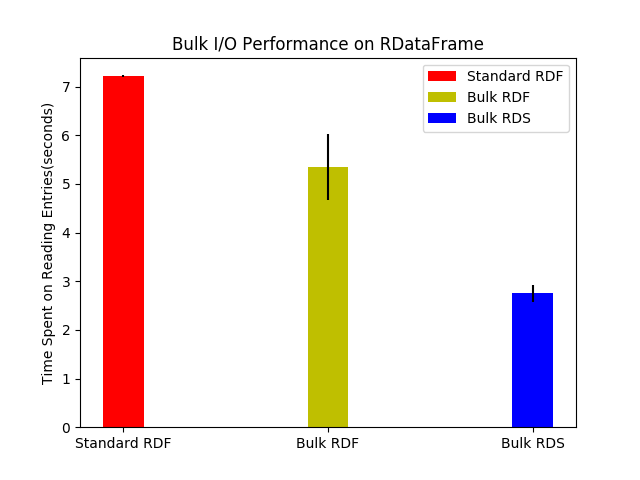
\includegraphics[height=4in, width=5in]{dataframe.png}
\vspace*{-2mm}
\caption{Performance improvements on RDataFrame with Bulk IO.}
\label{fig:rdataframe}
\end{figure}

Figure \ref{fig:rdataframe} shows the results of Bulk IO in RDataFrame. In this Figure \ref{fig:rdataframe}, standard RDF is the RDataFrame with normal ROOT IO library functions, while Bulk RDF is the results of reading events by RDataFrame and Bulk IO and Bulk RDS is the results that directly use RDataSource and Bulk IO. Bulk RDS outperforms standard RDF by more than 2 times. Since RDataFrame has extra overheads comparing to RDataSource (RDataFrame internally relies RDataSource), Bulk RDF runs slower than Bulk RDS, but still outperforms standard RDF.
